\documentclass[10pt,ignorenonframetext,]{beamer}
\setbeamertemplate{caption}[numbered]
\setbeamertemplate{caption label separator}{: }
\setbeamercolor{caption name}{fg=normal text.fg}
\beamertemplatenavigationsymbolsempty

\usepackage{pgfpages}
\pgfpagesuselayout{2 on 1}[a4paper,border shrink=5mm]

\usepackage{lmodern}
\usepackage{amssymb,amsmath}
\usepackage{ifxetex,ifluatex}
\usepackage{fixltx2e} % provides \textsubscript
\ifnum 0\ifxetex 1\fi\ifluatex 1\fi=0 % if pdftex
\usepackage[T1]{fontenc}
\usepackage[utf8]{inputenc}
\else % if luatex or xelatex
\ifxetex
\usepackage{mathspec}
\else
\usepackage{fontspec}
\fi
\defaultfontfeatures{Ligatures=TeX,Scale=MatchLowercase}
\fi
\usetheme{Madrid}
% use upquote if available, for straight quotes in verbatim environments
\IfFileExists{upquote.sty}{\usepackage{upquote}}{}
% use microtype if available
\IfFileExists{microtype.sty}{%
\usepackage{microtype}
\UseMicrotypeSet[protrusion]{basicmath} % disable protrusion for tt fonts
}{}
\newif\ifbibliography
\usepackage{longtable,booktabs}
\usepackage{caption}
% These lines are needed to make table captions work with longtable:
\makeatletter
\def\fnum@table{\tablename~\thetable}
\makeatother
\usepackage{graphicx,grffile}
\makeatletter
\def\maxwidth{\ifdim\Gin@nat@width>\linewidth\linewidth\else\Gin@nat@width\fi}
\def\maxheight{\ifdim\Gin@nat@height>\textheight0.8\textheight\else\Gin@nat@height\fi}
\makeatother
% Scale images if necessary, so that they will not overflow the page
% margins by default, and it is still possible to overwrite the defaults
% using explicit options in \includegraphics[width, height, ...]{}
\setkeys{Gin}{width=\maxwidth,height=\maxheight,keepaspectratio}

% Prevent slide breaks in the middle of a paragraph:
\widowpenalties 1 10000
\raggedbottom

\AtBeginPart{
\let\insertpartnumber\relax
\let\partname\relax
\frame{\partpage}
}
\AtBeginSection{
\ifbibliography
\else
\let\insertsectionnumber\relax
\let\sectionname\relax
\frame{\sectionpage}
\fi
}
\AtBeginSubsection{
\let\insertsubsectionnumber\relax
\let\subsectionname\relax
\frame{\subsectionpage}
}

\setlength{\parindent}{0pt}
\setlength{\parskip}{6pt plus 2pt minus 1pt}
\setlength{\emergencystretch}{3em}  % prevent overfull lines
\providecommand{\tightlist}{%
\setlength{\itemsep}{0pt}\setlength{\parskip}{0pt}}
\setcounter{secnumdepth}{0}

\title{Exploratory Factor Analysis}
\author{David Barron}
\date{Hilary Term 2017}

\begin{document}
\frame{\titlepage}

\section{Introduction}\label{introduction}

\begin{frame}{Introduction}

Exploratory factor analysis (EFA), often just called ``factor
analysis,'' is intended to help researchers understand the structure of
complex data, and possibly reduce the complexity by combining items that
can be considered to be indicators of the same underlying concept.

EFA refers to a set of procedures intended to determine the number of
distinct constructs needed to account for the pattern of observed
correlations among a set of measures. These constructs are called
\textbf{factors} (or more correctly ``common factors''), or sometimes
latent variables as distinct from the measured variables that are
actually observed.

The basic premise is that observed correlations among measured variables
are the result of the fact that they are influenced by the same common
factor. Hence, if we understand the relationships between common factors
and measured variables, we can potentially reduce the complexity of the
observed data.

The EFA model also assumes that observed measures are influenced by
\textbf{unique factors}, representing all sources of variance in each
measured variable that is not due to common factors. One such source is
measurement error, and indeed this is generally how unique factors are
conceptualised, as if there are systemmatic, unique factors that would
suggest a problem with the measure.

\end{frame}

\begin{frame}{Partitioning variance}

\[
\text{observed variance} = \text{common variance} + \text{unique variance}
\] \[
\text{unique variance} = \text{specific variance} + \text{error variance}
\] An important way of assessing an EFA model is the porportion of the
total variance accounted for by the common factors, which is called the
\textbf{communality.} \[
\text{communality} = \frac{\text{common variance}}{\text{observed variance}}
\]

\end{frame}

\section{Basic common factor model}\label{basic-common-factor-model}

\begin{frame}{Two common factors}

Graphical representation of a common factor model with two orthogonal
common factors and six measured variables.
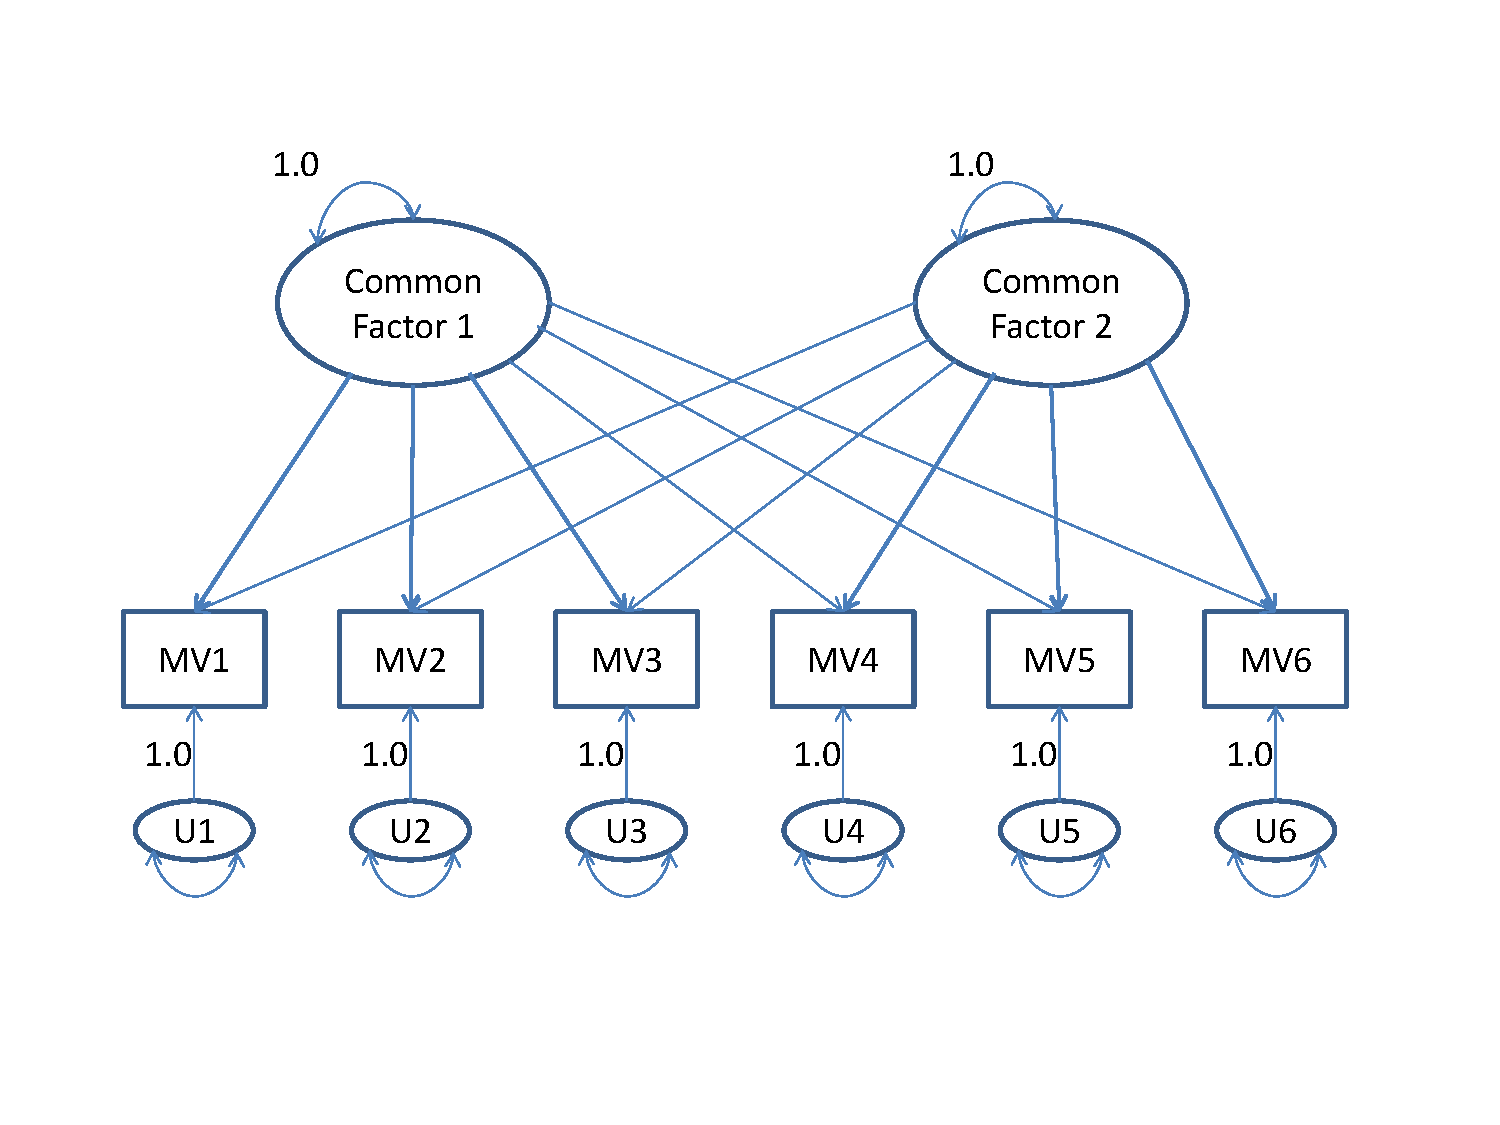
\includegraphics{BasicEFAPath.pdf}

\end{frame}

\begin{frame}{Path diagramme conventions}

It is conventional to represent factors/latent variables by circles or
ovals, measured variables by squares or rectangles, linear causal
relations by single-headed arrows, and covariances and variances by
double-headed arrows. Some relations and variances are constrained to
have the value 1.0. The common factors are not correlated with each
other (i.e., they are \emph{orthogonal}). The unique factors are
independent of each other.

\end{frame}

\begin{frame}{Correlation Structure Model}

\[
P = \Lambda \Phi \Lambda^T + D_\psi
\] \(P\) is the observed correlation matrix (a \(6 \times 6\) matrix in
our example): \[
P = \begin{pmatrix}
1.00 \\
\rho_{21} & 1.00 \\
\rho_{31} & \rho_{32} & 1.00 \\
\rho_{41} & \rho_{42} & \rho_{43} & 1.00 \\
\rho_{51} & \rho_{52} & \rho_{53} & \rho_{54} & 1.00 \\
\rho_{61} & \rho_{62} & \rho_{63} & \rho_{64} & \rho_{65} & 1.00 \\
\end{pmatrix}
\] \(\Lambda\) is the matrix of \emph{factor loadings}, the strength and
direction of the linear relationships between common factors and
measured variables: \[
\Lambda = \begin{pmatrix}
\Lambda_{11} & \Lambda_{12} \\
\Lambda_{21} & \Lambda_{22} \\
\Lambda_{31} & \Lambda_{32} \\
\Lambda_{41} & \Lambda_{42} \\
\Lambda_{51} & \Lambda_{52} \\
\Lambda_{61} & \Lambda_{62} \\
\end{pmatrix}
\]

\end{frame}

\begin{frame}{Correlation structure model, continued}

\(\Phi\) is the correlation matrix among the common factors: \[
\Phi = \begin{pmatrix}
1.00 & \Phi_{12}\\
\Phi_{21} & 1.00 \\
\end{pmatrix}
\] In the orthogonal model, \(\Phi_{21} = \Phi{12} = 0\), so this matrix
can be omitted. \(D_\Psi\) is the correlation matrix among the unique
factors. \[
D_\Psi = \begin{pmatrix}
D_{\Psi_{11}} & 0 & 0 & 0 & 0 & 0 \\
0 & D_{\Psi_{22}} & 0 & 0 & 0 & 0\\
0 & 0 & D_{\Psi_{33}} & 0 & 0 & 0 \\
0 & 0 & 0 & D_{\Psi_{44}} & 0 & 0 \\
0 & 0 & 0 & 0 & D_{\Psi_{55}} & 0 \\
0 & 0 & 0 & 0 & 0 & D_{\Psi_{66}} \\
\end{pmatrix}
\]

\end{frame}

\begin{frame}{Implications}

Consider two specific cases: \[
\rho_{11} = 1.00 = \Lambda_{11}\Lambda_{11} + \Lambda_{12}\Lambda_{12} + D_{\Psi_{11}}.
\] This implies that the variance of measureed variable 1 comes from
three sources, and the first term in the sum corresponds to the
proportion of the variance due to common factor 1, the second term to
the proportion of the variance due to common factor 2 and the third term
to that due to the unique factor.

\[
\rho_{21} = \Lambda_{21}\Lambda_{11} + \Lambda_{22}\Lambda_{12}.
\] This implies that the correlation between measured variables 1 and 2
is the sum of the product of common factor 1's loadings on MV1 and MV2,
and the product of common factor 2's loadings on MV1 and MV2. You can
see that if both MV1 and MV2 load highly on either common factor 1 or 2
(or both), then they will have a high correlation.

\end{frame}

\begin{frame}{Data considerations}

\begin{itemize}
\tightlist
\item
  When designing research with the expectation that EFA will be used, it
  is generally a good idea to plan to have at least 5 MVs per
  construct.\\
\item
  Keep measurement error to the minimum.
\item
  MVs should be interval variables (or a close approximation).
\item
  Sample sizes depend on the properties of the data.

  \begin{itemize}
  \tightlist
  \item
    Under optimal conditions (low measurement error, 3--5 MVs per
    construct), sample sizes of 100 should suffice.
  \item
    Under moderately good conditions, a sample size of 200 is adequate.
  \end{itemize}
\end{itemize}

\end{frame}

\begin{frame}{Common Factor Model or Principal Components Model?}

\small
There is a lot of confusion between these two. In fact, many people
report doing ``factor analysis'' when they in fact use principal
components analysis (PCA). It is widely believed that PCA is a ``type''
of factor analysis, but this is not the case. Although it may be true
that PCA often produces similar results to CFA, that is certainly not
always true. The main differences are:

\begin{itemize}
\tightlist
\item
  PCA was originally intended to reduce a set of MVs to the smallest set
  of scores that preserve as much information as possible. That is, it
  is about modelling the variances in MVs, not covariance among them.
\item
  Principal components were not intended to be thought of as
  corresponding to meaningful latent constructs.
\item
  Principal components do not distinguish between common and unique
  sources of variance in MVs.
\end{itemize}

You can think of PCA as being represented by: \[
P = \Lambda\Lambda^T, 
\] that is, assuming that there is no variance due to unique factors.

The attraction of PCA has been ease of computation, but this is no
longer a serious concern. I generally prefer CFA primarily because it
maps on to the idea that MVs are associated with theoretical, unobserved
constructs. We will look at both methods.

\end{frame}

\begin{frame}{Example data}

\scriptsize
How much of each of nine types of social support do each of 200
subjects, who are graduate students, provide to friends and family in an
average week? (1) the number of hugs the person gives (Hugs), (2) the
number of compliments the person gives (Comps), (3) the number of times
the person gives another person advice about his or her personal life
(PerAd), (4) the number of times the person invites someone to social
activities (SocAc), (5) the number of times the person provides some
type of professional advice (ProAd), (6) how often the person
participates in communal study sessions (i.e., studying in a group;
ComSt), (7) the number of times the person provides some form of
physical help, such as garden or house maintenance (PhyHlp), (8) how
often the person explicitly encourages others (Encour), and (9) how
often the person tutors other students on an academic subject (Tutor).

\begin{longtable}[]{@{}lllllllll@{}}
\toprule
Hugs & Comps & PerAd & SocAc & ProAd & ComSt & PhyHlp & Encour &
Tutor\tabularnewline
\midrule
\endhead
1.00 & 0.67 & 0.15 & 0.62 & 0.54 & 0.65 & 0.47 & 0.55 &
0.57\tabularnewline
0.67 & 1.00 & 0.25 & 0.58 & 0.51 & 0.64 & 0.42 & 0.54 &
0.49\tabularnewline
0.15 & 0.25 & 1.00 & 0.22 & 0.08 & 0.16 & 0.09 & 0.18 &
0.12\tabularnewline
0.62 & 0.58 & 0.22 & 1.00 & 0.41 & 0.56 & 0.34 & 0.45 &
0.35\tabularnewline
0.54 & 0.51 & 0.08 & 0.41 & 1.00 & 0.67 & 0.73 & 0.46 &
0.75\tabularnewline
0.65 & 0.64 & 0.16 & 0.56 & 0.67 & 1.00 & 0.60 & 0.54 &
0.67\tabularnewline
0.47 & 0.42 & 0.09 & 0.34 & 0.73 & 0.60 & 1.00 & 0.43 &
0.72\tabularnewline
0.55 & 0.54 & 0.18 & 0.45 & 0.46 & 0.54 & 0.43 & 1.00 &
0.41\tabularnewline
0.57 & 0.49 & 0.12 & 0.35 & 0.75 & 0.67 & 0.72 & 0.41 &
1.00\tabularnewline
\bottomrule
\end{longtable}

\end{frame}

\section{Number of common factors}\label{number-of-common-factors}

\begin{frame}{How many common factors?}

Although there are likely to be theoretical expectations about the
number of common factors, it is important that this be checked rather
than assumed. To obtain estimates of factor loadings in practice we have
to specify in advance how many common factors to include in the model,
and there are a range of methods intended to assess the appropriateness
of a choice. When making a choice, we need to find a model that:

\begin{enumerate}
\def\labelenumi{\arabic{enumi}.}
\tightlist
\item
  Does a good job of accounting for correlations among MVs;
\item
  Would do substantially worse with one fewer common factor;
\item
  Would not do substantially better with one more common factor;
\item
  All common factors can be readily interpreted and related to
  theoretical constructs.
\end{enumerate}

\end{frame}

\begin{frame}{Eigenvalues greater than one}

A very common method is based on the eigenvalues of the sample
correlation matrix. The rule (sometimes called the \emph{Kaiser
criterion}) is that the number of common factors required is equal to
the number of eigenvalues greater than 1. This rule has some logic when
it comes to PCA, but less so to CFA. It also performs poorly in
simulation studies.

\end{frame}

\begin{frame}{Scree test}

This involves producing a graph plotting the eigenvalues in descending
order. The graph is examined to find the number of eigenvalues before
the last major drop. This gives the number of factors to be selected. In
this example, the last major drop follows the second largest eigenvalue,
and so a two factor model would be used. It seems ad hoc, but in
practice often performs quite well.

\includegraphics[width=0.65\linewidth]{FactorAnlysis_files/figure-beamer/unnamed-chunk-2-1}

\end{frame}

\begin{frame}{Parallel analysis}

This method compares eigenvalues obtained from the sample correlation
matrix with eigenvalues obtained from random data. Random data is
generated with the same sample size and number of MVs and this is used
to obtain a correlation matrix. The random data eigenvalues are
typically averages over a number of simulations. The number of
eigenvalues from the sample data that are larger than the corresponding
eigenvalues from random data is the number of common factors.

\includegraphics[width=0.65\linewidth]{FactorAnlysis_files/figure-beamer/unnamed-chunk-4-1}

\end{frame}

\begin{frame}{Likelihood ratio test}

If we use maximum likelihood methods to obtain estimates of the factor
loadings, then it is possible to compare the goodness of fit of models
with different numbers of common factors using a likelihood ratio test.

\textbf{One-factor v. two-factor} \tiny

\begin{longtable}[]{@{}lrrrrrrrrrr@{}}
\toprule
& Model Df & ML Chisq & Delta Df & Delta Chisq & Pr(\textgreater{} Delta
Chisq) & Emp Chisq & Delta Emp Chisq & Pr(\textgreater{} Emp.Delta
Chisq) & BIC & Delta BIC\tabularnewline
\midrule
\endhead
efa1 & 19 & 17.1 & NA & NA & NA & 5.47 & NA & NA & -83.6 &
NA\tabularnewline
efa0 & 27 & 157.1 & 8 & 140 & 0 & 100.03 & 94.6 & 0 & 14.0 &
97.6\tabularnewline
\bottomrule
\end{longtable}

\normalsize

\textbf{Two-factor v. three-factor} \tiny

\begin{longtable}[]{@{}lrrrrrrrrrr@{}}
\toprule
& Model Df & ML Chisq & Delta Df & Delta Chisq & Pr(\textgreater{} Delta
Chisq) & Emp Chisq & Delta Emp Chisq & Pr(\textgreater{} Emp.Delta
Chisq) & BIC & Delta BIC\tabularnewline
\midrule
\endhead
efa2 & 12 & 8.65 & NA & NA & NA & 4.21 & NA & NA & -54.9 &
NA\tabularnewline
efa1 & 19 & 17.11 & 7 & 8.46 & 0.294 & 5.47 & 1.26 & 0.989 & -83.6 &
-28.6\tabularnewline
\bottomrule
\end{longtable}

\end{frame}

\begin{frame}{RMSEA}

Using a model fit index (more widely associated with the SEMs we will
discuss next week). The most common is the RMSEA (root mean squared
error of approximation):

\begin{longtable}[]{@{}ll@{}}
\toprule
Number of factors & RMSEA\tabularnewline
\midrule
\endhead
1 & 0.024\tabularnewline
2 & 0\tabularnewline
3 & 0\tabularnewline
\bottomrule
\end{longtable}

A general rule of thumb is that RMSEA lower than 0.08 are acceptable,
and ideally it should be below 0.05.

\end{frame}

\section{Rotation}\label{rotation}

\begin{frame}{Rotation}

Solutions to the factor analysis equations (i.e., sets of factor
loadings) are not unique. Although the solutions found by the fitting
algorithms are the best fit, there are an infite number of solutions
that have the same fit. So, how to select the best one? The process of
finding the best set of loadings is generally called \emph{rotation}
because you can think of it as rotating the axes that represent the
common factors about the origin. The ``best'' rotation will meet these
criteria:

\begin{itemize}
\tightlist
\item
  Each row should contain at least one value very close to 0;
\item
  Each column should contain at least \(m\) values close to 0, where
  \(m\) is the number of common factors;
\item
  Every pair of columns should have several rows with near zero values
  in one column but not the other;
\item
  Every pair of columns should have only a few rows with non-zero values
  in both columns.
\end{itemize}

\end{frame}

\begin{frame}[fragile]{Plot of factor loadings}

\begin{verbatim}
Loading required namespace: GPArotation
\end{verbatim}

\includegraphics[width=0.9\linewidth]{FactorAnlysis_files/figure-beamer/unnamed-chunk-7-1}

\end{frame}

\begin{frame}[fragile]{Factor loadings}

\tiny

\begin{verbatim}
Factor Analysis using method =  ml
Call: fa(r = efa.eg, nfactors = 2, n.obs = 200, rotate = "oblimin", 
    fm = "ml", normalize = TRUE)
Standardized loadings (pattern matrix) based upon correlation matrix
         ML1   ML2    h2   u2 com
Hugs    0.22  0.68 0.680 0.32 1.2
Comps   0.14  0.73 0.657 0.34 1.1
PerAd  -0.07  0.31 0.075 0.93 1.1
SocAc   0.00  0.74 0.552 0.45 1.0
ProAd   0.84  0.06 0.765 0.24 1.0
ComSt   0.48  0.47 0.705 0.30 2.0
PhyHlp  0.86 -0.04 0.695 0.30 1.0
Encour  0.21  0.52 0.435 0.56 1.3
Tutor   0.85  0.04 0.753 0.25 1.0

                       ML1  ML2
SS loadings           2.85 2.47
Proportion Var        0.32 0.27
Cumulative Var        0.32 0.59
Proportion Explained  0.54 0.46
Cumulative Proportion 0.54 1.00

 With factor correlations of 
     ML1  ML2
ML1 1.00 0.56
ML2 0.56 1.00

Mean item complexity =  1.2
Test of the hypothesis that 2 factors are sufficient.

The degrees of freedom for the null model are  36  and the objective function was  5.06 with Chi Square of  988
The degrees of freedom for the model are 19  and the objective function was  0.09 

The root mean square of the residuals (RMSR) is  0.02 
The df corrected root mean square of the residuals is  0.03 

The harmonic number of observations is  200 with the empirical chi square  5.47  with prob <  1 
The total number of observations was  200  with Likelihood Chi Square =  17.1  with prob <  0.58 

Tucker Lewis Index of factoring reliability =  1
RMSEA index =  0  and the 90 % confidence intervals are  NA 0.055
BIC =  -83.6
Fit based upon off diagonal values = 1
Measures of factor score adequacy             
                                                ML1  ML2
Correlation of scores with factors             0.95 0.92
Multiple R square of scores with factors       0.91 0.86
Minimum correlation of possible factor scores  0.81 0.71
\end{verbatim}

\end{frame}

\section{Example}\label{example}

\begin{frame}[fragile]{Maslach burnout inventory example}

\includegraphics{FactorAnlysis_files/figure-beamer/unnamed-chunk-9-1.pdf}

\begin{verbatim}
Parallel analysis suggests that the number of factors =  5  and the number of components =  NA 
\end{verbatim}

\end{frame}

\begin{frame}[fragile]{Factor loadings}

\tiny

\begin{verbatim}

Loadings:
     ML1    ML2    ML3   
l1    0.711 -0.120       
l2    0.814              
l3    0.766  0.106       
l8    0.868              
l12r  0.315  0.422       
l13   0.503         0.208
l14   0.557              
l20   0.436         0.209
l5                  0.514
l6    0.194         0.373
l10                 0.866
l11                 0.832
l15                 0.508
l16                 0.376
l22   0.163         0.359
l4r          0.503       
l7r          0.636       
l9r          0.648       
l17r         0.557       
l18r         0.536       
l19r         0.593       
l21r         0.542       

                 ML1   ML2   ML3
SS loadings    3.460 2.560 2.491
Proportion Var 0.157 0.116 0.113
Cumulative Var 0.157 0.274 0.387
\end{verbatim}

RMSEA: 0.004

\end{frame}

\begin{frame}{Factor loadings plot}

\includegraphics{FactorAnlysis_files/figure-beamer/unnamed-chunk-11-1.pdf}

\end{frame}

\end{document}
